\documentclass[10pt,a4paper,printanswers]{upmc} 

\usepackage[T1]{fontenc}
\usepackage[utf8]{inputenc}
%\usepackage[english]{babel}
\usepackage{amsmath}
\usepackage{amssymb}
\usepackage[ruled,vlined,linesnumbered]{algorithm2e}
\usepackage{mathtools}
\usepackage[usenames,dvipsnames]{xcolor}
\usepackage{framed}
\usepackage[framemethod=tikz]{mdframed}
\usepackage{listings}         

\global\mdfdefinestyle{graybox}{%
  linecolor=black,linewidth=1pt,%
  backgroundcolor=lightgray
}

\mdfdefinestyle{evaluation}{
    frametitlebackgroundcolor=black!15,
    frametitlerule=true,
    roundcorner=10pt,
    middlelinewidth=1pt,
    innermargin=0.5cm,
    outermargin=0.5cm,
    innerleftmargin=0.5cm,
    innerrightmargin=0.5cm,
    innertopmargin=\topskip,
    innerbottommargin=\topskip,
    frametitle={Milestone}
}

\usepackage[textwidth=18cm,textheight=25cm]{geometry}

\newcommand{\myline}{\noindent\makebox[\linewidth]{\rule{\textwidth}{0.7pt}}}
\newcommand{\mytilde}{\raise.17ex\hbox{$\scriptstyle\mathtt{\sim}$}}

\newcounter{mainmemorder}
\newcommand{\save}{\setcounter{mainmemorder}{\value{enumi}}}
\newcommand{\load}{\setcounter{enumi}{\value{mainmemorder}}}
\newcommand{\mytext}[1]{\colorbox{lightgray}{\texttt{#1}}}
\newcommand{\subsecline}{\texorpdfstring{\hrulefill}{}}

\newcommand{\Num}{Installation}
\newcommand{\UE}{\scriptsize M1 ISI/SAR/IPS\\ ROS \& experimental robotics}

\renewcommand*{\theenumi}{\#\thesection.\arabic{enumi}}

\title{ROS and experimental robotics.\\ \Num: Setting up you environment.}

\lstset{language=matlab,
  basicstyle=\small\sffamily,
  keywordstyle=\color{dblue}\bfseries,  
  commentstyle=\color{dred}\textit,
  stringstyle=\color{dgreen}\ttfamily,
  extendedchars=true,
  frame=single, 
  numbers=left,
  backgroundcolor=\color{lgray}
}

\begin{document}

\maketitle

In all the following, a Linux virtual machine will be used to work with ROS. It is based on the
Ubuntu 20.04 LTS (Long Term Support) distribution. The virtual machine will be launched by a host
machine, i.e.\ a machine with its own operating system, be it Linux, Windows or even macOS.
\textit{Nevertheless, we will assume here that the host machine is a Windows host, running with an
  up to date Windows 10 version.}

Using a virtual machine has several advantages, but the main point here is that the distributed
image already contains everything (mainly softwares and specific configurations) required to run a
Linux machine able to run ROS nodes and to control the Turtlebot robot. Almost no further
configuration is required and you will be able to use it almost immediately after downloading it.

\section{Installation of the virtual machine\subsecline}

First, you will have to download the virtualization platform. Multiple softwares exist to provide
hardware virtualization, like VirtualBox, VMware Fusion/Player/Workstation, Parallels, etc. In this
teaching unit, we will use the software \texttt{Workstation Workstation Player} (version 16.2.1 as
of 2022) provided by VMware. \texttt{VMware Workstation Player} allows you to run a second, isolated
operating system on a single PC. The use of this software is free for personal, non-commercial use,
and can be used either from a Windows or a Linux guest OS. Note that macOS users \textbf{with Intel
  processors} can also now download a free copy of \texttt{VMware Fusion} directly from the vmware
website. If using an Apple machine \textbf{with M1 processors}, VMware proposes a technical preview
of \texttt{VMware Fusion} which is still very limited, to date. If possible, it will be far easier
to work with a PC. Otherwise, \texttt{UTM} might be a good choice, and an image dedicated to this
software is also proposed, but to be used in last resort if it is not possible to use a PC instead.

\begin{enumerate}
  \item Download and install \texttt{VMware Workstation Player} on your Windows machine from
        \url{https://www.vmware.com/products/workstation-player.html}. You might have to create a
        free VMware account befor being able to download the software. There is no specific
        configuration here, so install \texttt{VMware Workstation Player} with the default proposed
        settings.
        \save
\end{enumerate}

Once installed, launch VMware  Workstation 16 from the Windows Start menu. The software window then
appears, with a Home menu from which you will be able to import an existing virtual machine.

\begin{enumerate}
  \load
  \item On Moodle, you will find an URL from which you will be able to download a pre-configured
        image for the Turtlebot Remote PC (\texttt{Turtlebot remote PC Noetic 2022.ova}). This
        image is quite big (about 10.1Go), so be patient and if possible download it from a good
        internet connection.
  \item Once downloaded to the \texttt{Download} folder, click on \texttt{Open a Virtual Machine} on
        the main window. From there, select the just downloaded Remote PC image, and click on
        \texttt{Open}. You will be asked to provide a name and the storage path for the new virtual
        machine. Select whatever you want here depending on your personal setup, as long as the disk
        where the virtual machine is hosted is big enough (you should have at least have 25GB free).
        %
        \begin{mdframed}[style=graybox]
          An error message might occur at this step ("The import failed because ... did not
          pass OVF specification conformance, etc.". Please click on \texttt{Retry} to overcome the
          issue.)
        \end{mdframed}
        The virtual machine is now imported and placed on the path specified before.
        %
  \item \textbf{Do not run immediatly the imported virtual machine now!}\\ A final step is now
        required before actually running the Turtlebot remote PC. Select the virtual machine from
        the main window, and then click on \texttt{Edit virtual machine settings}. A new window
        appears, containing all the virtual machine hardware specifications. From there, select the
        \texttt{Display} hardware section, and change the graphics memory size from 256MB to highest
        value, if possible.
\end{enumerate}

That's it! You should now have a ready to use Linux machine already configured with ROS and all
required software for the rest of this teaching unit.

\section{Configuration and test of the remote PC \subsecline}

It is now time to run the virtual machine. From the main window, select it and click on the
\texttt{Play} icon.
%
\begin{mdframed}[style=graybox]
  The virtual machine is configured with a NAT network interface, meaning than it is sharing the
  same network connection as the host, through a (non-visible) local network between the VM and the
  host. Consequently, the remote PC has its own local IP address, which is different from the host
  machine. This network configuration will have to be changed later to a bridged connection, so as
  to ease the connection betweem the VM and distant ROS nodes (i.e.\ communicate with the distant
  robot).
\end{mdframed}
The virtual machine now appears in a dedicated (small) window that can be resized or made full
screen. From now on, we will only work in this virtual machine, so make it at least full screen, or
better switch to \texttt{Full screen mode} from the dedicated button in the bar above the virtual
machine screen.

You should now have a full screen Linux machine running just like it was actually your main OS.
%
\begin{mdframed}[style=graybox]
  \begin{itemize}
    \item You might have some notifications about available software updates. You are free to
          install them as long as they \textbf{do not actually upgrade the OS major version itself!}
          (this should be the case) You might have to reboot the virtual machine to complete the
          update ;
    \item The virtual machine is launched as the user \texttt{turtle}, with password
          \texttt{turtlebot}.
  \end{itemize}
\end{mdframed}

The virtual machine is a standard Linux machine. If you are not familiar with Ubuntu, please pass
some time to explore the way it works. The main taskbar is already provided with shortcuts to
various already installed applications, see Figure~\ref{fig:taskbar}. Among them, there are some IDE
you can freely choose (Sublime Text, Spyder or Visual Studio Code) for the forthcoming Python
developments.
%
\begin{figure}[!h]
  \centering 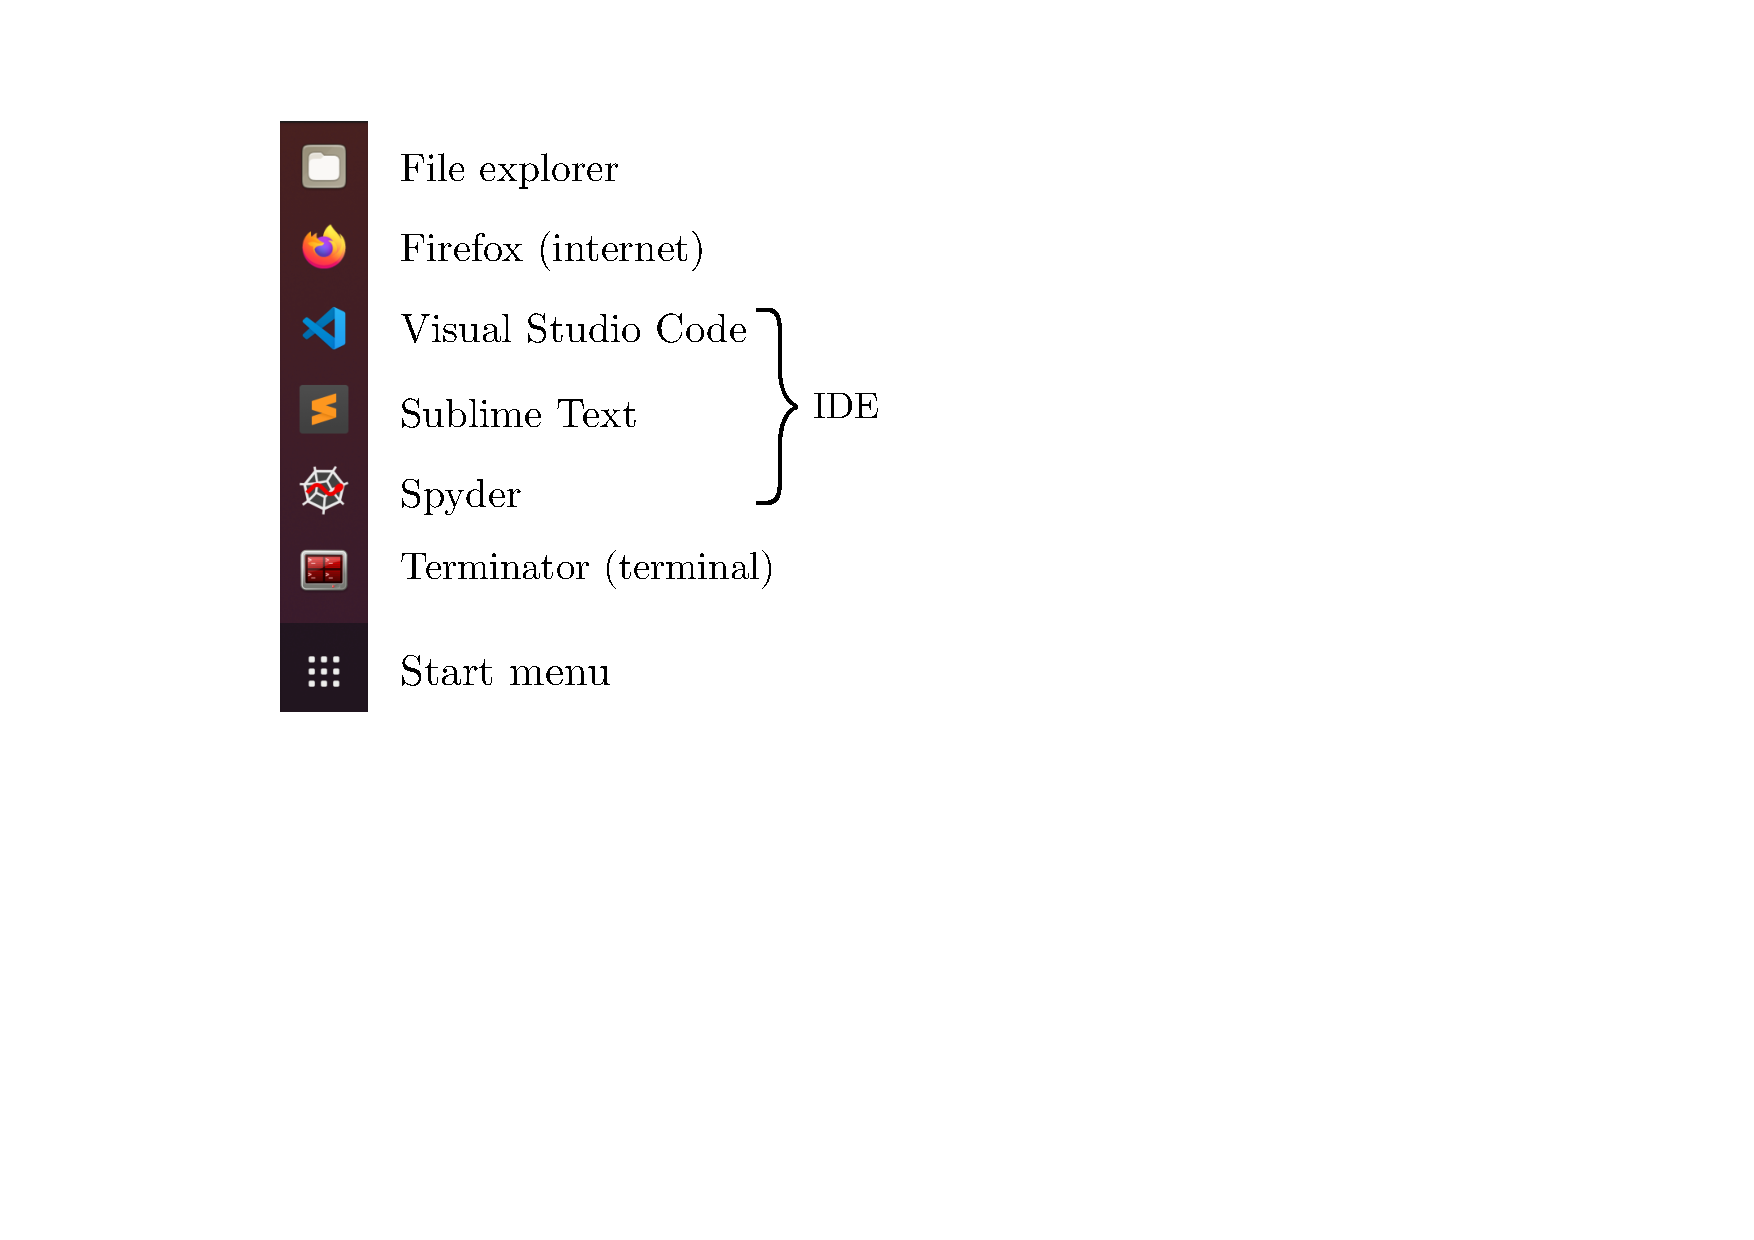
\includegraphics[width=5cm]{figures/taskbar.pdf}
  \caption{Default taskbar in the virtual machine.}
  \label{fig:taskbar}
\end{figure}

We will now test the virtual machine to verify it works correctly on your computer.


\begin{enumerate}
  \item Launch Terminator, a terminal application which gives you access to the computer shell.
        %
        \begin{mdframed}[style=graybox]
          A shell is a command-line interpreter that provides a command line user interface for
          Unix-like operating systems. The shell is both an interactive command language and a
          scripting language, and is used by the operating system to control the execution of the
          system using shell scripts.
          \begin{flushright}
            \textit{Bourne, Stephen R. (October 1983). "The Unix Shell". BYTE. p. 187.}
          \end{flushright}
        \end{mdframed}
        %
        Most of the commands you will be using in the following must be entered here. The terminal,
        and the shell running inside (which is \texttt{bash}), are probably one of the applications
        you will be using the most.

  \item For now, right click on the terminal, and choose \texttt{Split vertically} to open two
        different shells in the same terminal. Split again the right terminal in two horizontal
        windows. In the top right shell, run the following command:
        %
        \lstinputlisting[
          language=bash, % Use Perl functions/syntax highlighting
          frame=single, % Frame around the code listing
          showstringspaces=false, % Don't put marks in string spaces
          numbers=left, % Line numbers on left
          numberstyle=\tiny, % Line numbers styling
          basicstyle=\footnotesize,
        ]{code/turtlesim_test1.shell}

        Then, in the left shell, run the following command:
        \lstinputlisting[
          language=bash, % Use Perl functions/syntax highlighting
          frame=single, % Frame around the code listing
          showstringspaces=false, % Don't put marks in string spaces
          numbers=left, % Line numbers on left
          numberstyle=\tiny, % Line numbers styling
          basicstyle=\footnotesize,
        ]{code/turtlesim_test2.shell}

        A new blue window should appear, with a (randomly chosen) turtle in its center.
        Congratulation, you just launched your very first ROS node!

  \item Now, lets check if one can move the turtle in the window. In the bottom right shell, run
        the following command:
        \lstinputlisting[
          language=bash, % Use Perl functions/syntax highlighting
          frame=single, % Frame around the code listing
          showstringspaces=false, % Don't put marks in string spaces
          numbers=left, % Line numbers on left
          numberstyle=\tiny, % Line numbers styling
          basicstyle=\footnotesize,
        ]{code/turtlesim_test3.shell}

        You should now be able to move the turtle in its blue window by pressing the arrow keys on
        your keyboard (note that the terminal must be in the foreground so as to be able to capture
        the keys you are pressing. You might have to reduce the terminal window size to see the
        turtle actually moving on the other, blue, window).

\end{enumerate}

Close each program currently running in the 3 shells by pressing \texttt{Ctrl-C} on your keyboard
inside each terminal. If all the previous steps ran without any error, then you are now ready to
discover ROS and to work with the virtual machine.

\newpage

\end{document}
